\documentclass[11pt,ngerman,a4paper]{article}
%Gummi|061|=)
\usepackage{amsmath}
\usepackage{a4wide}
\usepackage{url}
\usepackage{amsthm}
\usepackage{amsbsy}
\usepackage{amssymb}
\usepackage[utf8]{inputenc}
\usepackage{rotating} 
\usepackage{here}
\usepackage{graphicx}
\usepackage{paralist}
\usepackage{selinput}
\usepackage[separate-uncertainty=true]{siunitx}
\usepackage{booktabs}
\sisetup{}
\SelectInputMappings{%
adieresis={ä},
germandbls={ß},
}
\title{\textbf{Versuch V703: Geiger-Müller-Zählrohr}}
\author{Martin Bieker\\
		Julian Surmann\\
		\\
		Durchgef\"{u}hrt am 27.05.2014\\
		TU Dortmund}
\date{}
\usepackage{graphicx}
\begin{document}
\renewcommand\tablename{Tabelle}
\renewcommand\figurename{Abbildung}
\maketitle
\thispagestyle{empty}
\newpage
\clearpage
\setcounter{page}{1}


\section{Einleitung}
Das Geiger-Müller-Zählrohr ist ein einfaches Messinstrument zur Messung der Intensität von ionisierender Strahlung. In diesem Versuch werden einige Kenndaten dieer Apparatur ermittelt.
\section{Theorie}
\subsection{Aufbau und Funktion} 
 Das Geiger-Müller-Zählrohr besteht aus einem Draht  mit Radius $r_a$, der sich in einem Metallzylinder mit Radius $r_k$ befindet (siehe Abb \ref{abb1}). 
\begin{figure}[htp]
\centering
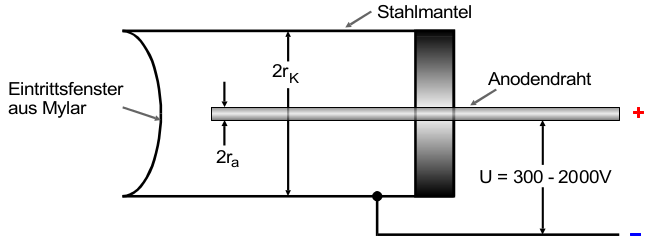
\includegraphics[scale=0.6]{/home/martin/Dokumente/SS14/Praktikum/V703/abb1.png}
\caption{Aufbau eines Geiger-Müller-Zählrohrs. [1]}
\label{abb1}
\end{figure} 
Zwischen diesen Elementen wird eine elektrische Spannung von \SI{300}{\volt} bist \SI{2000}{\volt} angelegt. Auf diese Weise entsteht zwischen Anodendraht und Kathodenzylinder ein radial-symmetrisches Feld. Der Innenraum ist mit einem  Edelgasgemisch gefüllt. Da im Innenraum ein Unterdruck herrschen soll, ist das Zählrohr an den Enden verschlossen. An einer Seite befindet sich aber eine dünner Mylarfolie, damit  auch $\alpha$ und $\beta$-Teilchen in den Innenraum eindringen können.
 
 \noindent
 Wenn Strahlung in das Zählrohrvolumen eindringt, werden die Edelgasatome ionisiert. Da die Energie der Strahlung ein Vielfaches der Ionsierungsenergie ist, können mehrere Atome ionsiert werden, bis die Strahlung vollständig absorbiert ist. Die durch die Ionisierungsakte freigesetzte Elektronen werden durch das elektrische Feld  zum Anodendraht beschleunigt.

Die nach der ersten Ionisation ablaufende Prozesse hänegn sehr stark von der Zylinder anliegenden Spannung ab. In Abbildung \ref{abb2} wird die Anzahl der pro einfallendem Teilchen erzeugten Elektronen-Ionen-Paare als Funktion der am Zählrohr angelegten Spannung dargestellt.
\begin{figure}[htp]
\centering
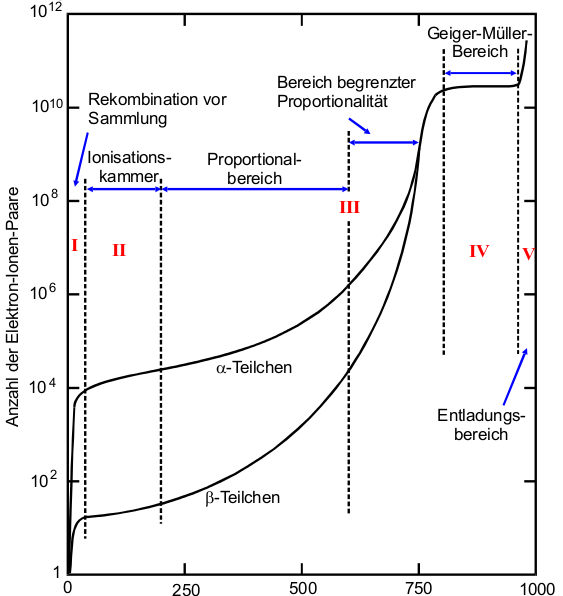
\includegraphics[scale=0.5]{/home/martin/Dokumente/SS14/Praktikum/V703/abb2.png}
\caption{Anzahl der pro Teilchen erzeugten Ladungen als Funktion der Betriebsspannung.[1]}
\label{abb2}
\end{figure}
Ist das elektrische Feld nicht sehr stark, werden rekombinieren mit den Ionen bevor sie den Anodendraht erreichen. Dies entspricht Bereich I in der Abbildung. Wird die Spannung erhöht erreichen mehr Elektronen den Draht bevor sie rekombinieren können. In diesem Spannungsbereich (II in der Abbildung) wird das Zählrohr als Ionisationskammer betrieben. Bei weiterer Erhöhung der Spannung sind  die beschleunigten Elektronen auf Grund ihrer Energie in der Lage weitere Atome zu ionisieren. Es entsteht eine so genannte Townsend-Lawine. Es kann nun ein Ladungsimpuls gemessen werden, welcher von der Energie der Einfallenden Strahlung abhängt. In diesem Bereich können mit dem Zählrohr sowohl die Intensität, als auch die Energie einer Strahlungsquelle gemessen werden. Daher wird die Apparatur in diesem Bereich als Proportionalitätszährohr bezeichnet. 
Steigt die Spannung weiter an, sind die Spannungsimpulse nicht mehr von der Teilchenenergie abhängig (Bereich IV). Bei der Ionisation durch die Elektronen entstehen auf Grund des starken elektrischen Feldes UV-Quanten. Da diese ungeladen sind, verursachen sie auf ganzer Länge des Zählrohrs weitere Ionisationslawinen auslösen. In diesem Spannungsbereich wird ein Geiger-Müller-Zählrohr betrieben.
Bei weiterer Steigerung der Spannung wird die Apparatur durch Dauerentladungen zerstört.
\subsection{Charektersitik}
Die Anzahl der Ladungsimulse bei gegebener Zeit und Quellenintensität als Funktion der anliegenden Spannung wird als Charakteristik des Zählrohres. Diese ist beispielhaft in Abbildung \ref{abb3} dargestellt.
\begin{figure}[htp]
\centering
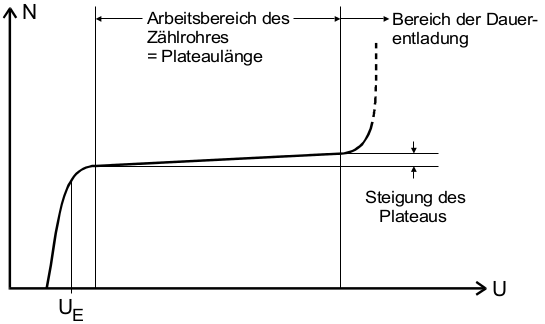
\includegraphics[scale=0.60]{/home/martin/Dokumente/SS14/Praktikum/V703/abb3.png}
\caption{Charakterisktik eines Zählrohrs. [1]}
\label{abb3}
\end{figure}
Das in dieser Abbildung dargestellte Plateau ist der eigentliche Messbereich des Geiger-Müller-Zählählrohrs.Die die Länge und die Steigung des Plateaus sind wichtige Kennziffern für die Qualität der Apparatur.
 
\subsection{Totzeit und Nachtentladungen}

Die, bei den Ionisationsvorgängen entstehenden, positiven Edelgasionen haben im Vergleich zu den Elektronen eine sehr große Masse. Daher wandern diese nur langsam zur Kathode. Durch die im Zylinder vorherrschende positive Ladungsdichte schirmt das Feld indes Anodendrahts ab. Aus diesem Grund können für eine gewisse Zeit $T$ nach einem Impuls keine weiteren Teilchen erkannt werden. Dieser Effekt wird als Totzeit bezeichnet. Erst nachdem alle positiven Ionen neutralisiert wurden, erreichen die Ladungsimpulse ihre volle Stärke. Dieser Zeitraum heißt Erholungszeit $T_E$.

\noindent
Treffen die Edelgasionen auf den Kathodenzylinder lösen diese dort Elektronen aus der Metalloberfläche. Diese Elektronen können weitere Ionisations- und Endladungslawinen auslösen. Diese Nachentladungen verfälschen das Messergebnis, da dann bei einem Ladungsimpuls nicht unterschieden werden kann, ob dieser von einem Teilchen oder von einem Elektron aus dem Kathodenmaterial ausgelöst wurde. Um die Entstehung solcher Nachentladungen zu verhindern, wird dem Gas im Zählrohr eine geringe Menge eines Alkohols hinzugefügt. Diese relativ großen Moleküle nehmen die Energie der Ionen auf und wandeln diese in thermische Schwingungen um. Auf diese Weise können keine Elektronen aus der Metalloberfläche ausgelöst werden.
\section{Durchführung}
Der Versuch ist wie in Abbildung \ref{abb4} gezeigt aufgebaut.
\begin{figure}[htp]
\centering
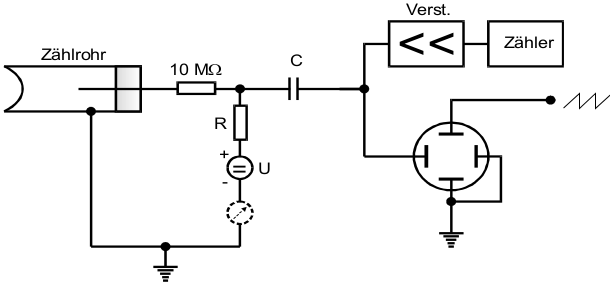
\includegraphics[scale=0.5]{/home/martin/Dokumente/SS14/Praktikum/V703/abb4.png}
\caption{Schaltplan für Messungen am Geiger-Müller-Zählrohr. [1]}
\label{abb4}
\end{figure}
Das Zählrohr ist an eine variable Spannungsquelle angeschlossen. In einen hochohmigen Widerstand werden die Ladungsimpulse in Spannungsimpulse gewandelt und über einen Kondensator ausgekoppelt. Diese Impulse werden dann einerseits verstärkt und gezählt und andererseits mit einem Oszilloskop sichtbar gemacht.
\subsection{Aufnahme der Charakteristik}
Zur Aufnahme der Charakteristik wird ein $\beta$-Strahler vor dem Zählrohr angebracht und die Zählrate in Abhängigkeit von der Spannung gemessen. Dabei wird die Spannung von \SI{300}{\volt} bis \SI{700 }{\volt} in \SI{20}{\volt} variiert. Damit der relative Fehler der Messung unter \SI{1}{\percent} bleibt, wird der Messzeitraum
\[
\Delta t
\]
so gewählt, dass die Anzahl der gezählten Ereignisse
\[
N \geq \num{10000}
\]
ist. Zusätzlich wird mit einem Strommessgerät der durch das Zählrohr fließende Strom gemessen, um später die pro Teilchen freigesetzte Ladungsmenge zu bestimmen. 
\subsection{Oszillographische Messungen}
Zunächst sollen die Nachentladungen am Oszilloskop sichtbar gemacht werden. Dazu wird zunächst die Intensität der $\beta$-Quelle soweit gesenkt, dass die Wahrscheinlichkeit für zwei direkt aufeinander folgende Teilchen vernachlässigbar klein ist. Danach wird das Zählrohr einmal mit einer Spannung betrieben bei der Nachtentladungen unwahrscheinlich sind. Danach wird die Zählrohrspannung auf ihr Maximum von \SI{700}{\volt} erhöht.

\noindent
Danach soll die Totzeit und die Erholungszeit mit Hilfe des Oszilloskops bestimmt werden. Dazu wird eine hohe Stahlintensität gewählt. Es ergibt sich ein Oszillogramm wie in Abbildung \ref{abb5}.
\begin{figure}[htp]
\centering
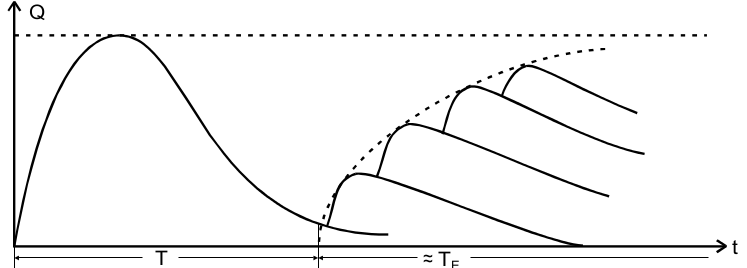
\includegraphics[scale=0.55]{/home/martin/Dokumente/SS14/Praktikum/V703/abb5.png}
\caption{Schematische Darstellung eines Oszilogramms zur Bestimmung von Tot- und Erhohlungszeit. [1]}
\label{abb5}
\end{figure}
Aus diesem können Totzeit und die Erholungszeit grob abgelesen werden.
\subsection{Bestimmung der Totzeit mit der Zwei-Quellen-Methode}
Zur Bestimmung der Totzeit mit der Zwei-Quellen-Methode wird zunächst die Zählrate mit einer Quelle $N_1$ bestimmt. Danach wird eine zweite Quelle in den Versuchsaufbau eingebracht und die Zählrate beider Quellen $N_{1+2}$ ermittelt. Im Anschluss wird die erste Quelle entfernt und die Zählrate nur in Anwesenheit der zweiten Quelle $N_2$ gemessen. Die Totzeit $T$ ist dann durch 
\[
T \approx \frac{N_1 + N_2 - N_{1+2}}{2N_1N_2}
\]
gegeben.
 
\section{Auswertung}
\begin{table}
\centering
\begin{tabular}{SSSSS}
\toprule
{U[V]} &{ N} &{ t[s]} &{ $I\left[\frac{1}{s}\right]$} &{ $\sigma_{I,rel}$[\%] }\\
\midrule
300.0 & 0.0 & 100.0 & 0 & nan\\
320.0 & 13617.0 & 250.0 & 54.5+-0.5 & 0.86\\
340.0 & 11192.0 & 200.0 & 56.0+-0.5 & 0.95\\
360.0 & 11231.0 & 200.0 & 56.2+-0.5 & 0.94\\
380.0 & 11601.0 & 200.0 & 58.0+-0.5 & 0.93\\
400.0 & 11410.0 & 200.0 & 57.0+-0.5 & 0.94\\
420.0 & 11459.0 & 200.0 & 57.3+-0.5 & 0.93\\
440.0 & 11496.0 & 200.0 & 57.5+-0.5 & 0.93\\
460.0 & 11433.0 & 200.0 & 57.2+-0.5 & 0.94\\
480.0 & 11379.0 & 200.0 & 56.9+-0.5 & 0.94\\
500.0 & 11457.0 & 200.0 & 57.3+-0.5 & 0.93\\
520.0 & 11437.0 & 200.0 & 57.2+-0.5 & 0.94\\
540.0 & 11376.0 & 200.0 & 56.9+-0.5 & 0.94\\
560.0 & 11564.0 & 200.0 & 57.8+-0.5 & 0.93\\
580.0 & 11620.0 & 200.0 & 58.1+-0.5 & 0.93\\
600.0 & 11333.0 & 200.0 & 56.7+-0.5 & 0.94\\
620.0 & 11382.0 & 200.0 & 56.9+-0.5 & 0.94\\
640.0 & 11449.0 & 200.0 & 57.2+-0.5 & 0.93\\
660.0 & 11414.0 & 200.0 & 57.1+-0.5 & 0.94\\
680.0 & 11507.0 & 200.0 & 57.5+-0.5 & 0.93\\
700.0 & 11642.0 & 200.0 & 58.2+-0.5 & 0.93\\
\bottomrule
\end{tabular}
\label{}
\caption{Messdaten und Fehlerangabe}
\end{table}


\begin{table}
\centering
\begin{tabular}{SSSS}
\toprule
{N} &{ t[s]} &{ $I\left[\frac{1}{s}\right]$} &{ $\sigma_{I,rel}$[\%] }\\
\midrule
17483.0 & 200.0 & 87.4+-0.7 & 0.76\\
20229.0 & 200.0 & 101.1+-0.7 & 0.70\\
13280.0 & 1000.0 & 13.28+-0.12 & 0.87\\
\bottomrule
\end{tabular}
\label{}
\caption{}
\end{table}


\section{Quellen}
\begin{enumerate}[{[}1{]}]
\item Entnommen der Praktikumsanleitung \textit{} der TU Dortmund. \\
Download am 01.06.14 unter:\\
 \url{http://129.217.224.2/HOMEPAGE/PHYSIKER/BACHELOR/AP/SKRIPT/V703.pdf}
\end{enumerate}

\section{Anhang}
\begin{itemize}
\item Tabellen
\item Auszug aus dem Messheft
\end{itemize}
\end{document}
